%
% grenze.tex -- Die Grenze der elementaren Integration
%
% (c) 2026 Baris Catan, OST Ostschweizer Fachhochschule
%
% !TEX root = ../../buch.tex
% !TEX encoding = UTF-8
%
\section{Die Grenze der elementaren Integration
\label{elliptisch:section:grenze}}
\kopfrechts{Die Grenze}

In der Einleitung haben wir behauptet, das Integral
\eqref{elliptisch:equation:umfang} habe keine elementare
Stammfunktion.
In diesem Abschnitt wollen wir genauer untersuchen, wo die Grenze
zwischen elementar und nicht elementar verläuft.
Es geht dabei durchgehend um Integranden der Form
$R\bigl(x,\sqrt{p(x)}\bigr)$, also um rationale Funktionen in $x$
und in der Wurzel aus einem Polynom $p(x)$.

\subsection{Der quadratische Fall
\label{elliptisch:subsection:quadratisch}}
\index{Euler-Substitution}%
Für ein Polynom vom Grad höchstens $2$ ist die Lage vollständig
geklärt.
Wir schreiben
\begin{equation}
\vartheta = \sqrt{ax^2 + bx + c}
\label{elliptisch:equation:theta}
\end{equation}
und betrachten Integranden, die rational in $x$ und $\vartheta$
sind.
Mithilfe der Euler-Substitution $\vartheta = \sqrt{a}\,x + t$ (für
$a > 0$) lässt sich $x$ als rationale Funktion von $t$ schreiben.
Quadrieren der Substitutionsgleichung und Vergleichen mit
$\vartheta^2 = ax^2 + bx + c$ ergibt
\begin{equation}
x
=
\frac{c - t^2}{2\sqrt{a}\,t - b},
\label{elliptisch:equation:eulersubst}
\end{equation}
und damit werden auch $dx$ und $\vartheta$ rational in $t$
(Kapitel~\ref{chapter:ratint}).
Der Integrand wird dadurch zu einer rationalen Funktion von $t$
allein, und rationale Funktionen sind stets elementar integrierbar.
Die Partialbruchzerlegung erzeugt nur Bausteine, deren
Stammfunktionen Logarithmen, Potenzen und Arkustangens sind.
Ein Resultat dieser Rechnung ist
\begin{equation}
\int \frac{dx}{\vartheta}
=
\frac{1}{\sqrt{a}}\,
\log\bigl(2ax + b + 2\sqrt{a}\,\vartheta\bigr),
\label{elliptisch:equation:quadratisch}
\end{equation}
zu finden in
Abschnitt~\ref{buch:intalg:wurzel:subsection:stammfunktiontheta}.
Die Gestalt der rechten Seite ist typisch für diesen Fall.
Sie besteht aus einem konstanten Vorfaktor und dem Logarithmus
eines Elements des Funktionenkörpers.
Das ist genau die Form \eqref{elliptisch:equation:liouville}, die der Satz 
von Liouville für eine elementare
Stammfunktion verlangt, hier mit $v_0 = 0$ und einem einzigen
Logarithmusterm.
Steht unter der Wurzel ein Polynom vom Grad $\le 2$, so ist das
Integral immer elementar lösbar.

\subsection{Definition des elliptischen Integrals}
Ab Grad $3$ versagt dieses Verfahren, der Grund dafür wird in
Abschnitt~\ref{elliptisch:subsection:wurzelbleibt} deutlicher.
\begin{definition}
\index{elliptisches Integral}%
Ein \emph{elliptisches Integral} ist ein Integral der Form
\begin{equation}
\int R\bigl(x, \sqrt{p(x)}\bigr)\,dx,
\label{elliptisch:equation:definition}
\end{equation}
wobei $R$ eine rationale Funktion in zwei Variablen ist und $p$ ein
Polynom vom Grad $3$ oder $4$ ohne mehrfache Nullstellen.
\end{definition}
Die Bedingung an die Nullstellen ist wesentlich.
Hätte $p$ eine doppelte Nullstelle, also
$p(x) = (x-\alpha)^2 q(x)$, dann liesse sich der Faktor aus der
Wurzel ziehen, $\sqrt{p(x)} = |x-\alpha|\sqrt{q(x)}$, und der
effektive Grad sänke auf höchstens $2$.
Wir wären damit wieder im quadratischen Fall des vorangegangenen
Abschnitts.
Die Grade $3$ und $4$ stehen in der Definition zusammen, weil sie
dieselbe Schwierigkeitsklasse bilden.
Ist $\deg p = 4$ und $\alpha$ eine Nullstelle von $p$, so schreiben
wir $p(x) = (x-\alpha)q(x)$ mit $\deg q = 3$ und substituieren
$x = \alpha + 1/u$.
Wegen $dx = -du/u^2$ und
\begin{equation}
p\biggl(\alpha+\frac{1}{u}\biggr)
=
\frac{1}{u}\,q\biggl(\alpha+\frac{1}{u}\biggr)
=
\frac{Q(u)}{u^4},
\qquad
Q(u) = u^3\,q\biggl(\alpha+\frac{1}{u}\biggr),
\label{elliptisch:equation:gradreduktion}
\end{equation}
mit einem Polynom $Q$ vom Grad höchstens $3$ kürzt sich das $u^2$
aus der Wurzel gegen dasjenige in $dx$, und es bleibt
\begin{equation}
\frac{dx}{\sqrt{\smash[b]{\underbrace{p(x)}_{\text{Grad } 4}}}}
=
-\frac{du}{\sqrt{\smash[b]{\underbrace{Q(u)}_{\text{Grad } 3}}}}.
\label{elliptisch:equation:gradreduziert}
\end{equation}
\vspace{0.6ex}

\noindent
Aus dem Grad $4$ ist damit Grad $3$ geworden, und dieselbe
Substitution führt umgekehrt von Grad $3$ auf Grad $4$.
Polynome vom Grad $5$ und mehr führen auf die
\emph{hyperelliptischen} Integrale, die wir hier nicht behandeln.
\index{hyperelliptisches Integral}%
Abbildung~\ref{fig:elliptisch:gradskala} fasst diese Einteilung
zusammen.
\begin{figure}
	\centering
	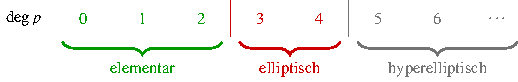
\includegraphics[width=0.9\textwidth]{papers/elliptisch/images/gradskala.pdf}
	\caption{Der Grad des Polynoms $p$ unter der Wurzel entscheidet
	über die Lösbarkeit.
	Bis Grad $2$ ist das Integral elementar, bei den Graden $3$ und
	$4$ elliptisch, ab Grad $5$ hyperelliptisch.}
	\label{fig:elliptisch:gradskala}
\end{figure}
%
Den Namen haben die elliptischen Integrale vom geometrischen
Problem, zu dem wir jetzt zurückkehren, nämlich der Bogenlänge
der Ellipse.

\subsection{Das Ellipsenumfangsintegral}
In der Einleitung haben wir den Umfang der Ellipse auf das Integral
\eqref{elliptisch:equation:umfang} gebracht.
Warum es in die Definition \eqref{elliptisch:equation:definition}
fällt, sehen wir nach einer weiteren Substitution.
Das Kriterium verlangt eine rationale Variable, wir setzen daher
$x = \sin t$ mit $dt = dx/\sqrt{1-x^2}$ und erhalten mit den neuen
Grenzen $0$ und $1$
\begin{equation}
U
=
4a \int_0^1 \frac{\sqrt{1-k^2x^2}}{\sqrt{1-x^2}}\,dx
=
4a \int_0^1
\frac{\sqrt{(1-x^2)(1-k^2x^2)}}{1-x^2}\,dx.
\label{elliptisch:equation:umfangsubstituiert}
\end{equation}
Unter der Wurzel steht mit
\begin{equation}
p(x)
=
(1-x^2)(1-k^2x^2)
=
k^2x^4 - (1+k^2)x^2 + 1
\label{elliptisch:equation:gradvier}
\end{equation}
ein Polynom vom Grad $4$ in $x$, das für $0 < k < 1$ keine
mehrfachen Nullstellen hat.
Somit erfüllt das Ellipsenumfangsintegral genau die Definition
\eqref{elliptisch:equation:definition} und ist ein elliptisches
Integral.
Zu beachten ist noch, dass der Integrand in
\eqref{elliptisch:equation:umfangsubstituiert} bei $x = 1$ eine
Singularität hat.
Das Integral ist dort uneigentlich, aber konvergent, da der Zähler
wie $\sqrt{1-x}$ verschwindet.

\subsection{Warum die Wurzel bleibt
\label{elliptisch:subsection:wurzelbleibt}}

Mit der Einordnung als elliptisches Integral ist noch nichts über
die Lösbarkeit gesagt.
Die Definition \eqref{elliptisch:equation:definition} beschreibt eine
Bauform, keine Unmöglichkeit.
Das sieht man an
\begin{equation}
\int \frac{p'(x)}{2\sqrt{p(x)}}\,dx
=
\sqrt{p(x)},
\label{elliptisch:equation:zufallelementar}
\end{equation}
denn der Integrand ist rational in $x$ und $\sqrt{p(x)}$, das
Polynom $p$ darf Grad $4$ haben und quadratfrei sein, und trotzdem
ist die Stammfunktion elementar.
Die Frage nach der elementaren Lösbarkeit muss also für jedes
Integral einzeln gestellt werden.

Warum sie im quadratischen Fall stets zu bejahen ist, liegt tiefer
als in der Rechnung von
Abschnitt~\ref{elliptisch:subsection:quadratisch}.
Die Gleichung $\vartheta^2 = ax^2+bx+c$ beschreibt einen
Kegelschnitt, und die Euler-Substitution
\eqref{elliptisch:equation:eulersubst} ist seine rationale
Parametrisierung.
Sie drückt $x$ und $\vartheta$ rational durch $t$ aus, und umgekehrt
ist $t = \vartheta - \sqrt{a}\,x$ rational in $x$ und $\vartheta$.
Genau diese beidseitig rationale Zuordnung überträgt den
Integranden in eine rationale Funktion von $t$.
Für $\deg p \in \{3,4\}$ ist die Kurve $y^2 = p(x)$ dagegen eine
elliptische Kurve, und eine solche besitzt keine rationale
Parametrisierung \cite{elliptisch:geddes}.
\index{elliptische Kurve}%
Es gibt also keine Substitution, die den Integranden rational macht.
Der Weg des quadratischen Falls ist damit versperrt, und die Wurzel
bleibt stehen.

Dass kein anderer Weg zum Ziel führt, folgt daraus noch nicht.
Der Satz von Liouville
\eqref{elliptisch:equation:liouville} liefert an dieser Stelle eine
notwendige Bedingung.
Er sagt, welche Gestalt eine elementare Stammfunktion haben müsste,
und der Nachweis der Nichtexistenz besteht darin, diese Gestalt zu
widerlegen.
Für algebraische Erweiterungen ist das erheblich aufwendiger als für
logarithmische und exponentielle.
Polynome lassen sich dort nicht mehr eindeutig faktorisieren, der
euklidische Algorithmus fällt weg, und an seine Stelle treten
Divisoren aus der algebraischen Geometrie
\cite{elliptisch:geddes}.
Abschnitt~\ref{buch:intalg:risch:algebraisch} beschreibt, was dazu
nötig wäre, und verzichtet aus demselben Grund auf die Ausführung.
Wir übernehmen das Resultat.
%
% memeFIG.tex
%
% (c) 2026 Prof Dr Andreas Müller
%
\begin{figure}
\centering
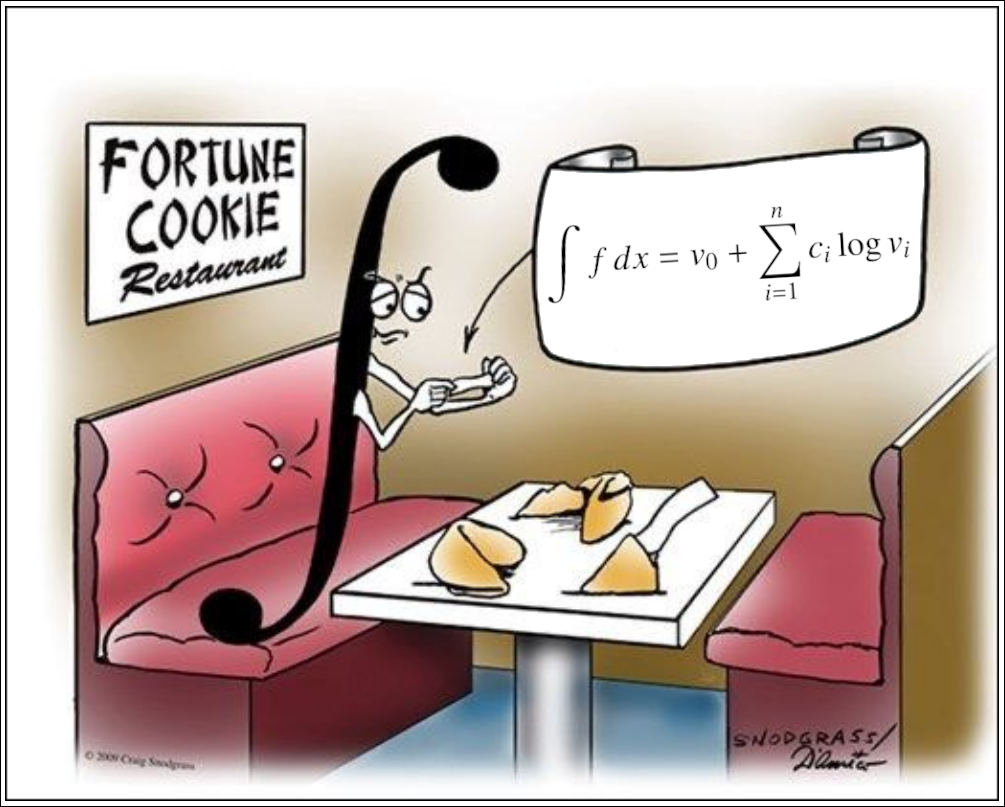
\includegraphics[width=\textwidth]{papers/elliptisch/images/meme2.png}
\caption{Das Prinzip von Liouville (Satz~\ref{elliptisch:satz:liouville})
charakterisiert die Funktionen, die eine elementare Stammfunktionen haben.
Dieses Meme stellt es als ein Fortune Cookie dar, welches dem Integral
vorhersagt, ob es mit einem Integranden Glück haben wird wird.
\label{elliptisch:meme}}
\end{figure}


\begin{satz}
\label{elliptisch:satz:nichtelementar}
Für $0 < k < 1$ besitzt keines der beiden Integrale
\begin{equation}
\int \frac{dx}{\sqrt{(1-x^2)(1-k^2x^2)}}
\qquad\text{und}\qquad
\int \frac{\sqrt{1-k^2x^2}}{\sqrt{1-x^2}}\,dx
\label{elliptisch:equation:nichtelementar}
\end{equation}
eine elementare Stammfunktion.
\end{satz}
Eine Beweisskizze und die Verweise auf die Spezialliteratur geben
Geddes, Czapor und Labahn \cite{elliptisch:geddes}.
Das zweite Integral in \eqref{elliptisch:equation:nichtelementar} ist
bis auf den Faktor $4a$ genau der Umfang der Ellipse aus
\eqref{elliptisch:equation:umfangsubstituiert}.
Die Frage vom Anfang des Kapitels ist damit beantwortet, wenn auch
negativ.
Eine elementare Formel für den Ellipsenumfang gibt es nicht, und die
Suche danach war von Beginn an aussichtslos.
Was bleibt, ist der Schritt, den wir schon bei der Fehlerfunktion
gesehen haben.
Das Integral bekommt einen Namen und wird selbst zur Funktion.
